\section{Software Agents}
\label{sec:agents}

\begin{figure}
    \centering
    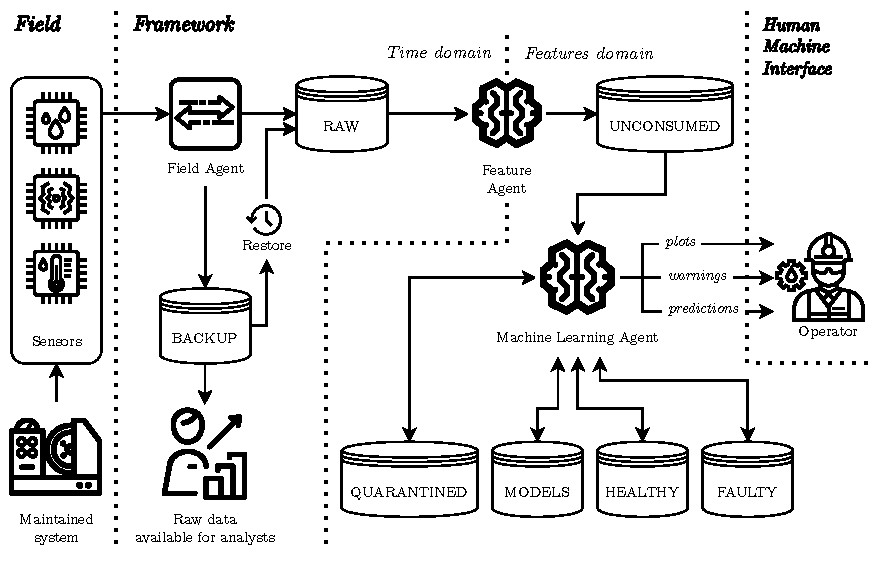
\includegraphics[width=\textwidth]{images/Framework/Framework_structure.pdf}
    \caption{Framework logical structure}
    \label{fig:Framework_structure}
\end{figure}

In the previous sections, the software agents were mentioned as the main actors in the \gls{glo:frmwrk}. This section will provide a more detailed description of the software agents, their role and their interaction with the environment and the data, following the flow from the hardware through the time-series, the \gls{glo:feature} domain to the \gls{ml} algorithms. The reference layout is the one in \autoref{fig:Framework_structure}. 

Software \gls{glo:agent}s are autonomous programs that perform a specific task in a cycle. In the proposed \texttt{\gls{glo:python}} implementation, the agents are classes that are instanced and run in a loop.

\subsection{Field Agent}
\label{subsec:FieldAgent}
\begin{figure}
    \centering
    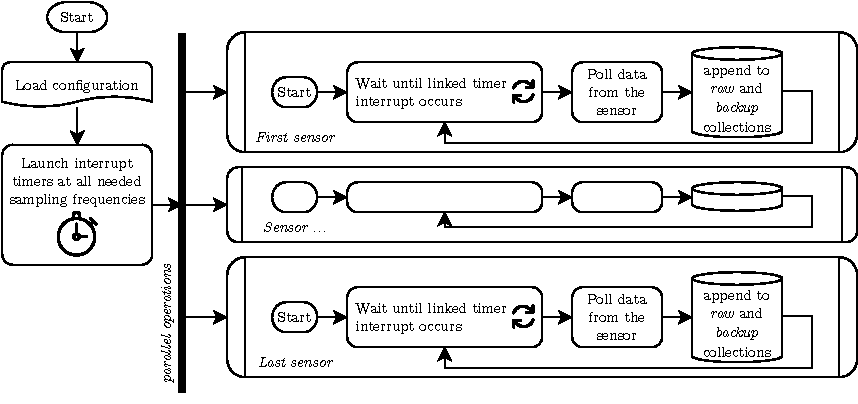
\includegraphics[scale=1]{images/Framework/Field_Agent_flowchart.pdf}
    \caption{Field Agent flowchart}
    \label{fig:Field_Agent_flowchart}
\end{figure}

The \gls{glo:fieldagent} is the interface between the hardware and the software. It is responsible for the acquisition of the data from the sensors and the communication with the database. Since some \gls{glo:feature}s are related to the spectrum of the data, a precise and fixed sampling frequency is needed. Hence, the \gls{fieldAg} must incorporate a synchronization with the \gls{adc}. It stores data in the \emph{raw} collection and the \emph{backup} collection. In \autoref{fig:Field_Agent_flowchart}, the flow of operations is shown as a flowchart, emphasizing the importance of the synchronization with the \gls{adc}. This software agent has not been implemented in \texttt{\gls{glo:python}}, because the experimental validation of this work, as it will be described in \autoref{sec:Validation}, has been performed directly on the \gls{glo:edge} platform. During the tests on the publicly available datasets, an abstract version of the \gls{fieldAg} has been used, that reads the data from the \gls{csv} files.


\subsection{Feature Agent (\gls{fa})}
\label{subsec:FeatureAgent}
\begin{figure}
    \centering
    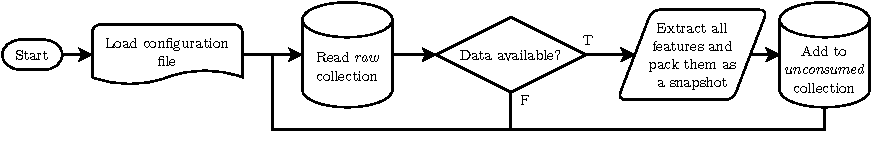
\includegraphics[width=\textwidth]{images/Framework/FA_flowchart.pdf}
    \caption{Feature Agent flowchart}
    \label{fig:FA_flowchart}
\end{figure}

The \gls{fa} is responsible for the \gls{glo:feature} extraction from the raw data. It reads the data from the \emph{raw} collection, extracts the \gls{glo:feature}s and stores them in the \emph{unconsumed} collection. The flow of operation is shown in \autoref{fig:FA_flowchart}. The \gls{fa} is implemented in \texttt{\gls{glo:python}} and it is a class that has been designed to be easily expandable and configurable. The methods implemented in the \gls{fa} class are shown in \autoref{tab:FA_methods}.


\begin{longtable}{p{0.4\textwidth}p{0.5\textwidth}}
    \caption{\gls{fa} class implemented methods\label{tab:FA_methods}}\\ 
    \toprule
    \textbf{Method} & \textbf{Description} \endfirsthead
    \hline
    readFromRaw & reads a \gls{glo:snap} from the raw collection and stores it in the instance self \\
    extractFeatures & extract all the \gls{glo:feature}s from the current \gls{glo:snap}s, for all the sensors \\
    extractTimeFeautures & extract~mean,~rms, P2P, std, skewness and kurtosis, based on the config file for the specified sensor \\
    extractFreqFeautures & extract the wavelet coefficients for the specified sensor, up to the configured depth \\
    deleteFromraw & delete current snap record from the \emph{raw} collection \\
    writeToUnconsumed & write the extracted \gls{glo:feature}s to the \emph{unconsumed} collection \\
    initialize\_barPlotFeatures & initializes the bar plot of the \gls{glo:feature}s that is shown to the user \\
    barPlotFeatures & updates the bar plot with new \gls{glo:feature}s \\
    run & perform the agent operations in a loop. idle until new data are available in \emph{raw} collection \\
    \bottomrule
\end{longtable}
    

\subsection{Machine Learning Agent (\gls{mla})}
\label{subsec:MLA}
The \gls{mla} is responsible for the training and the evaluation of the \gls{ml} models. It reads the data from the \emph{unconsumed} collection, evaluates the \gls{glo:snap} and stores the result in the \emph{models} collection, it also constantly updates the information about the novelty or fault metric to the user. The flow of operation is shown in \autoref{fig:MLA_structure}. The methods implemented in the \gls{mla} class are shown in \autoref{tab:MLA_methods}.

This agent is designed to be configured as a \gls{nd} or \gls{fd} agent with just one \gls{glo:hyperparameter}. If it is instanced for \gls{nd}, it uses the healthy collection as a training dataset, if it is instanced for \gls{fd} it uses the faulty collection. The metric used to evaluate the \gls{glo:snap}s is the novelty metric for \gls{nd} and the fault metric for \gls{fd}. According to the procedure defined in \autoref{alg:eval_new_snapshot}.

\begin{figure}[htbp]
    \centering
    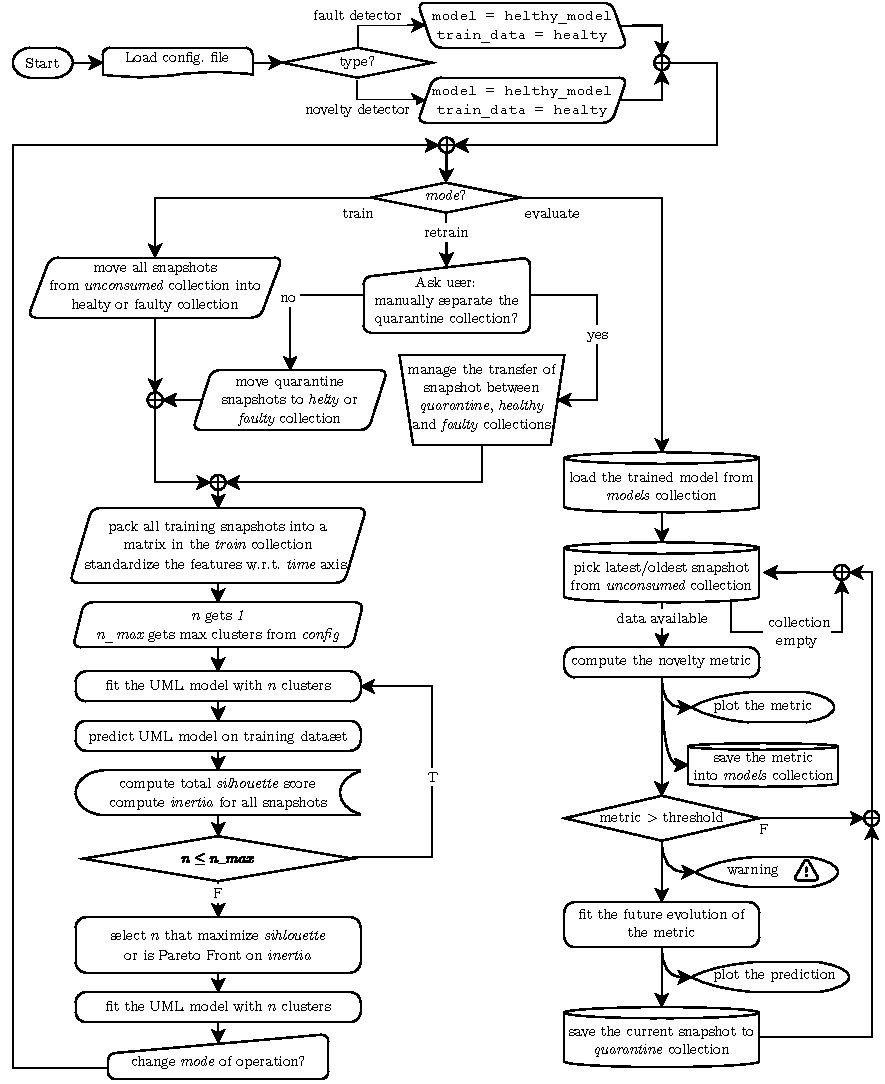
\includegraphics[width=\textwidth]{images/Framework/MLA.pdf}
    \caption{Machine Learning Agent flowchart. When it is instanced for \gls{nd}, the \gls{mla} uses the healthy collection as a training dataset, when it is instanced for \gls{fd} it uses the faulty collection.}
    \label{fig:MLA_structure}
\end{figure}


\begin{longtable}{p{0.4\textwidth}p{0.5\textwidth}}
    \caption{\gls{mla} class implemented methods\label{tab:MLA_methods}}\\ 
    \toprule
    \textbf{Method} & \textbf{Description} \endfirsthead 
    \hline
    run & run the \gls{mla} according to its current state \\
    evaluate & evaluate the current \gls{glo:snap} based on the novelty or the fault metric, according to the type of instance \\
    predict & fits the novelty metric with a degradation curve to predict the future evolution~ \\
    mark\_snap\_evaluated & set the evaluated flag to true for the current \gls{glo:snap} \\
    delete\_evaluated\_snap & remove the evaluated \gls{glo:snap}s from the \emph{unconsumed} collection \\
    scale\_\gls{glo:feature}s & scales the \gls{glo:feature}s of the current \gls{glo:snap} according to the standard scaler used during the training procedure \\
    evaluate\_error & compute the novelty or fault metric for the current \gls{glo:snap}, according to the type of instance \\
    calculate\_train\_cluster\_dist & compute the radiuses of the \gls{glo:clust}s during the training procedure \\
    prepare\_train\_data & performs the preprocessing of the data before training the model \\
    pack\_train\_data & pack the training \gls{glo:snap} in a matrix \\
    \_\_move\_to\_train & move an entire collection of \gls{glo:snap}s to the training collection \\
    standardize\_\gls{glo:feature}s & make all the \gls{glo:feature}s in the training matrix have zero mean and unitary variance \\
    save\_\gls{glo:feature}s\_limits & save the unscaled bounds of the training \gls{glo:feature}s \\
    save\_StdScaler & store the standard scaler instance in \gls{glo:pickle} into the database \\
    retrieve\_StdScaler & restore the standard scaler instance in \gls{glo:pickle} from the database \\
    save\_KMeans & store the model instance in \gls{glo:pickle}  \\
    retrieve\_KMeans & restore the model instance in \gls{glo:pickle}  \\
    \_append\_\gls{glo:feature}s & append the current \gls{glo:feature}s in a document \\
    train & performs the training of the \gls{glo:clust}ing models \\
    evaluate\_silhouette & compute the silhouette score of the training set \gls{glo:snap}s \\
    \_\_plot\_silhouette & plots the silhouette score against the number of \gls{glo:clust}s \\
    evaluate\_inertia & compute the inertia score of the training set \gls{glo:snap}s \\
    \_\_plot\_inertia & plots the inertia score against the number of \gls{glo:clust}s \\
    packFeaturesMatrix & format all the training \gls{glo:feature}s as a matrix \\
    retrain & perform a new training of the models \\
    \bottomrule
    \end{longtable}
    
\newpage
\subsection{Configuration of the \gls{glo:frmwrk}}
All the configurations described in this chapter are stored in the \texttt{config.yaml} file. This file is read by the agents at the beginning of their execution. The configuration file is divided into sections by topic: database, models etc. The \autoref{tab:yaml} shows the structure of the configuration file.


\begin{longtable}{>{\hspace{0pt}}m{0.26\linewidth}>{\hspace{0pt}}m{0.113\linewidth}>{\hspace{0pt}}m{0.569\linewidth}}
  \caption{Structure of the \gls{glo:frmwrk} configuration file.\label{tab:yaml}}\\ 
  \toprule
  \rowcolor[rgb]{0.929,0.929,0.923}\textbf{Field} & \textbf{Type} & \textbf{Description} \endfirsthead 
  \hline
  Database & structure & Database configuration \\
  \rowcolor[rgb]{0.929,0.929,0.923}$\dots$/URI & string & MongoDB URI \\
  $\dots$/DB & string & Database name \\
  \rowcolor[rgb]{0.929,0.929,0.923}$\dots$/Collection & structure & Collections configuration \\
  $\dots$/$\dots$/Backup & string & Backup collection name \\
  \rowcolor[rgb]{0.929,0.929,0.923}$\dots$/$\dots$/Raw & string & Raw data collection name \\
  $\dots$/$\dots$/Unconsumed & string & Unconsumed data collection name \\
  \rowcolor[rgb]{0.929,0.929,0.923}$\dots$/$\dots$/Healthy & string & Healthy data collection name \\
  $\dots$/$\dots$/Healthy\_train & string & Healthy data collection packed for training (some healthy data are not used if not novelty) \\
  \rowcolor[rgb]{0.929,0.929,0.923}$\dots$/$\dots$/Quarantined & string & Quarantined data collection name \\
  $\dots$/$\dots$/Faulty & string & Faulty data collection name \\
  \rowcolor[rgb]{0.929,0.929,0.923}$\dots$/$\dots$/Faulty\_train & string & Faulty data collection packed for~training (some faulty data are not used if not novelty) \\
  $\dots$/$\dots$/Models & string & Models collection name \\
  \rowcolor[rgb]{0.929,0.929,0.923}Sensors & structure & Sensors configuration \\
  $\dots$/Sensor 1/Name & string & Sensor 1 name \\
  \rowcolor[rgb]{0.929,0.929,0.923}$\dots$/$\dots$/Features & structure & Features configuration of this sensor \\
  $\dots$/$\dots$/$\dots$/Wavelet & bool & Enable or disable wavelet decomposition for the considered sensor \\
  \rowcolor[rgb]{0.929,0.929,0.923}$\dots$/$\dots$/$\dots$/Mean & bool & Enable or disable mean \gls{glo:feature} for the considered sensor \\
  $\dots$/$\dots$/$\dots$/\gls{rms} & bool & Enable or disable \gls{rms} \gls{glo:feature} for the considered sensor \\
  \rowcolor[rgb]{0.929,0.929,0.923}$\dots$/$\dots$/$\dots$/P2P & bool & Enable or disable P2P \gls{glo:feature} for the considered sensor \\
  $\dots$/$\dots$/$\dots$/Std & bool & Enable or disable Standard deviation \gls{glo:feature} for the considered sensor \\
  \rowcolor[rgb]{0.929,0.929,0.923}$\dots$/$\dots$/$\dots$/Skew & bool & Enable or disable skewness \gls{glo:feature} for the considered sensor \\
  $\dots$/$\dots$/$\dots$/Kurt & bool & Enable or disable kurtosis \gls{glo:feature} for the considered sensor \\
  \rowcolor[rgb]{0.929,0.929,0.923}$\dots$/$\dots$ & $\dots$ & $\dots$ \\
  $\dots$/Sensor n/Name & string & Sensor $n$ name \\
  \rowcolor[rgb]{0.929,0.929,0.923}$\dots$/Sensor\_n/Features & structure & Features configuration of this sensor \\
  $\dots$/Sensor n/$\dots$ & $\dots$ & $\dots$ \\
  \rowcolor[rgb]{0.929,0.929,0.923}Wavelet & structure & Wavelet Packet Decomposition configuration \\
  $\dots$/Type & string & Type of wavelet to be used (ex. db10, Moore, etc.) \\
  \rowcolor[rgb]{0.929,0.929,0.923}$\dots$/Mode & string & Mode of decomposition (ex. Symmetric) \\
  $\dots$/Level & int & Depth of the decomposition tree (No. of \gls{glo:feature}s~$=2^\text{Level}$) \\
  \rowcolor[rgb]{0.929,0.929,0.923}Model & structure & Models configuration \\
  $\dots$/Max \gls{glo:clust}s & int & Maximum number of \gls{glo:clust}s to attempt during \gls{glo:clust}ing \\
  \rowcolor[rgb]{0.929,0.929,0.923}$\dots$/Max iterations & int & Maximum iterations of the \gls{uml} algorithm \\
  $\dots$/queue & int & Number of \gls{rul} predictions to keep in memory \\
  \rowcolor[rgb]{0.929,0.929,0.923}$\dots$/Plot size & int & Number of Novelty Metric values to be kept in memory for plotting \\
  Novelty-Fault & structure & Configuration of the novelty or fault detection \\
  \rowcolor[rgb]{0.929,0.929,0.923}$\dots$/Threshold & float & Novelty - Fault detection threshold \\
  $\dots$/\gls{rul} Threshold & float & Novelty - Fault threshold for \gls{rul} predictions \\
  \rowcolor[rgb]{0.929,0.929,0.923}$\dots$/Fit points & int & Number of samples used for fitting the prediction curve \\
  $\dots$/Outlier filter & int & Number of consecutive outliers to filter \\
  \rowcolor[rgb]{0.929,0.929,0.923}$\dots$/Regressor & string & Type of curve to fit (exp or scipy to select the closed form solution or the iterative solution) \\
  Log & string & Path where to store the logs of the \gls{glo:frmwrk} \\
  \bottomrule
  \end{longtable}
  

\subsection{Command Line Interface (\gls{cli})}
\label{subsec:CLI}

To ease the interaction with the user, a \gls{cli} has been implemented. It relies on the \texttt{click} and \texttt{typer} libraries for \texttt{\gls{glo:python}}. The \gls{cli} allows the user to instance the agents, to configure the \gls{glo:frmwrk}, to monitor the agents and to interact with the database. All the commands are provided with a help message that can be accessed by typing \texttt{{-}{-}help} after the command, as shown in \autoref{fig:cli} for the command \texttt{run-machine-learning-agent}.
The commands implemented in the \gls{cli} are shown in \autoref{tab:CLI_commands}.

\begin{figure}[h!]
  \centering
  \includegraphics[width=\textwidth]{images/Framework/cli.png}
  \caption{Command Line Interface help message}
  \label{fig:cli}
\end{figure}

\begin{longtable}{p{0.4\textwidth}p{0.5\textwidth}}
    \caption{\gls{cli} implemented commands\label{tab:CLI_commands}}\\ 
    \toprule
    \textbf{Command} & \textbf{Description} \endfirsthead 
    \hline
    copy-collection            &Move all the documents from one collection to another\\
    create-empty-db            &Create an empty database in MongoDB. The database should not exist already. It is configured according with "config.yaml" file.\\
    ims-converter              &Transfer the data from the gls{ims} textual files into the MongoDB database in a suitable way.\\
    fault-indicator            &This function plots the fault metric.\\
    novelty-indicator          &This function plots the novelty metric.\\
    move-collection            &Move all the documents from one collection to another\\
    plot-\gls{glo:feature}s              &Plot the \gls{glo:feature}s of the last \gls{glo:snap} in the UNCONSUMED collection\\
    run-\gls{glo:feature}-agent          &Run the Feature Agent - takes the last \gls{glo:snap} from RAW collection, extracts \gls{glo:feature}s and writes them to UNCONSUMED collection\\
    run-machine-learning-agent &Run the Machine Learning Agent \\
    \bottomrule
    \end{longtable}